%%
%% UnBTeX: A class for bachelor, master, and doctoral thesis at the
%% University of Brasilia (UnB), Brazil
%% Version 1.5.2 2024/07/04
%% Copyright (C) 2021-2024 by Henrique C. Ferreira <hcferreira@unb.br>
%%
%% This class file may be distributed and/or modified under the conditions
%% of the LaTeX Project Public License, either version 1.3 of this license
%% or (at your option) any later version. The latest version of this
%% license is in:
%% 
%%    http://www.latex-project.org/lppl.txt
%% 
%% and version 1.3 or later is part of all distributions of LaTeX version
%% 2005/12/01 or later.
%%
%% This file is a template for use with the UnBTex class
%% To compile the document you should call pdflatex, bibtex, pdflatex
%% 

\documentclass[
    % -- Opção da classe memoir -- https://www.ctan.org/pkg/memoir
    oneside, % Caso queira imprimir em frente e verso, use twoside
    % -- Opção da classe abntex2 -- https://www.ctan.org/pkg/abntex2
    sumario=tradicional, % Remova esta opção para sumário padrão ABNT
    % -- Selecione o idioma no qual o trabalho será escrito
    %idioma=brazil, % Para texto principal em português
    idioma=english, % Para texto principal em inglês  
    % -- Selecione o estilo das referências bibliográficas
    bib=alf, % Bibliografia nas normas da ABNT, estilo autor-data
    %bib=num, % Bibliografia nas normas da ABNT, estilo numérico
    % -- Opções de idiomas para pacotes utilizados -- Não alterar
    english, % Para hifenização de palavras em inglês
    brazil % Para hifenização de palavras em português
    ]{unbtex}

% ---
% Pacotes básicos (Adicione outros pacotes necessários para o seu trabalho)
\usepackage{tikz}
\usepackage{pgfplots}
\usepackage{booktabs}
\usepackage{array}
\usepackage{caption}
\usepackage{xcolor}
% ---
\usepackage{longtable} % Pacote para tabelas que ocupam mais de uma página
\usepackage{rotating} % Pacote para girar tabelas (e outros objetos)
% ---

% ---
% Compila o índice
% ---
\makeindex
% ---

% ---
% Compila a nomenclatura
% ---
\makenomenclature
% ---

% ---
% Diretório das figuras
\graphicspath{{unbtex-example/figuras}}
% --- 

% ------------------------------------------------------------------------
% ------------------------------------------------------------------------
% Informações do trabalho
% ------------------------------------------------------------------------
% ------------------------------------------------------------------------

% ---
% Título
% ---
\titulo{Secure remote control UAV system based on chaotic cryptography in hardware} % No idioma principal do texto
% Insira \\ caso queira forçar quebras de linha no título
% Não utilize caixa alta para o título do trabalho e nem das seções (com exceção de siglas)
% ---
\tituloestrangeiro{} % Escreva aqui título em português se o trabalho for escrito em inglês (caso contrário, deixe vazio)
% ---

% ---
% Autores
% ---
\autori[]{Arthur}{Lima} % \autori[]{Nome}{Sobrenome}
% No caso de nomes como Carlos de Souza, utilize \autori[]{Carlos de}{Souza} (e não \autori[]{Carlos}{de Souza})
% ---
\autorii[]{}{} % Deixe os argumentos vazios se não tiver segundo autor
% ---

% ---
% Código Cutter para a ficha catalográfica
% Gerado a partir da entrada <Sobrenome, Nome> (do primeiro autor) no site https://www.tabelacutter.com/
% ---
\numerocutter{} % Para não imprimir o código na ficha catalográfica, deixe o argumento vazio
%\numerocutter{769} % Prencher o argumento do comando apenas com os números gerados
% ---

% ---
% Orientadores
% ---
\orientador[Orientador]{Prof. Dr.}{Jones Yudi}{Silva} % Para alterar o gênero, basta trocar Orientador por Orientadora
% ---
\coorientador[Coorientador]{Prof. Dr.}{Janier}{Arias-Garcia} % Deixe os argumentos para nome e sobrenome vazios se não tiver coorientador 
% ---

% ---
% Informações do trabalho
% ---
\tipotrabalho{Dissertação de Mestrado} % Dissertação de Mestrado; Tese de Doutorado (em português, mesmo que o trabalho seja em inglês)
%\tipotrabalho{Tese de Doutorado}
% ---
\tipocurso{Programa de Pós Graduação em Sistemas Mecatrônicos} % Nome do curso de graduação ou do programa de pós-graduação, em português
%\tipocurso{Programa de Pós-Graduação em Engenharia Elétrica}
% ---
% Texto que aparece na folha de rosto e na folha de aprovação
\preambulo{Trabalho da Disciplina de Dissertação em Engenharia Mecatrônica 2024/1.} 
%\preambulo{Tese de Doutorado submetida ao Programa de Pós-Graduação em Engenharia Elétrica da Universidade de Brasília como parte dos requisitos necessários para obtenção do grau de Doutor.}
% Consulte a secretaria/coordenação do curso para saber o que deve ser escrito no preâmbulo. Use português mesmo que o trabalho seja em inglês.
% ---
% Informação adicional para ser impressa na folha de rosto
\publicacao{} % Deixe o argumento vazio caso não haja
%\publicacao{Publicação PPGEE 201/23} % Também imprime as informações do trabalho no topo da página da ficha catalográfica
% ---

% ---
% Instituição
% ---
%\instituicao[Universidade de Brasília]{Faculdade de Tecnologia}{} % Use português mesmo que o trabalho seja em inglês
\instituicao[Universidade de Brasília]{Faculdade de Tecnologia}{Programa de Pós Graduação em Sistemas Mecatrônicos} % Caso queira incluir o departamento da unidade acadêmica
% ---

% ---
% Local e data da defesa
% ---
\local{Brasília}
\dia{4}
\mes{julho}
\ano{2024}
% ---

% ---
% Membros da banca
% ---
%
\membrodabancai{Prof. Dr. Jones Yudi Silva,\\ UnB/FT/ENM} % Membro 1 - Geralmente é o orientador
\membrodabancaifuncao{Orientador} % Em português, mesmo que o trabalho seja em inglês.
\membrodabancaii{Prof. Dr. Janier Arias-Garcia,\\ UFMG/ENE} % Membro 2
\membrodabancaiifuncao{Coorientador}
\membrodabancaiii{} % Membro \membrodabancaiiifuncao{Examinador interno}
\membrodabancaiv{} % Deixe vazio se não tiver o quarto membro
\membrodabancaivfuncao{Examinador externo}
\membrodabancav{} % Deixe vazio se não tiver o quinto membro
\membrodabancavfuncao{Examinador externo}
\signlinewidth{9cm}
% ---

% ---
% Resumo em português
% ---
\begin{Resumo}
Este documento exemplifica a elaboração de trabalho acadêmico (trabalho de conclusão de curso, dissertação e tese) a partir da classe UnB\TeX, uma extensão da classe \abnTeX\ para a Universidade de Brasília (UnB). Além de apresentar comandos básico de \LaTeX\ para inclusão de equações, tabelas e figuras, o documento mostra como utilizar pacotes adotados pela classe UnB\TeX\ para gerar referências bibliográficas, listas símbolos, caixas para teoremas e algoritmos, dentre outros elementos úteis ou obrigatórios para trabalhos acadêmicos. Espera-se que este documento facilite o uso da classe UnB\TeX\ na elaboração de trabalhos de alta qualidade gráfica mesmo por usuários com pouca experiência em \LaTeX.
\end{Resumo}
% ---

% ---
% Resumo em inglês
% ---
\begin{Abstract}
This is the english abstract.
\end{Abstract}
% ---

% ---
% Palavras-chave (pelo menos três devem ser informadas)
% ---
\pchavei{Palavra chave 1}
\kwordi{Keyword 1}
\pchaveii{Palavra chave 2}
\kwordii{Keyword 2}
\pchaveiii{Palavra chave 3}
\kwordiii{Keyword 3}
\pchaveiv{Palavra chave 4} % Deixe vazio se não tiver
\kwordiv{Keyword 4} % Deixe vazio se não tiver
\pchavev{} % Deixe vazio se não tiver
\kwordv{} % Deixe vazio se não tiver
% ---

% ---
% Agradecimentos
% ---
% Idioma usado nos agradecimentos (pode ser em português, mesmo que o trabalho seja em inglês)

% Dedicatória
% ---

% Primeiro autor
%\begin{DedicatoriaAutorI}
%Este trabalho é dedicado às crianças adultas que,\\
%quando pequenas, sonharam em se tornar cientistas.
%\end{DedicatoriaAutorI}

% Segundo autor
%\begin{DedicatoriaAutorII}
%Dedicatória do segundo autor.
%\end{DedicatoriaAutorII}
% ---

% ---
% Epígrafe
% ---
\begin{Epigrafe}
\vspace*{\fill}
\begin{flushright}
    \textit{``If you find that you're spending almost all your time on theory,\\
    start turning some attention to practical things;\\
    it will improve your theories.\\
    If you find that you're spending almost all your time on practice,\\
    start turning some attention to theoretical things;\\
    it will improve your practice.''\\
    (Donald Knuth)}
\end{flushright}
\end{Epigrafe}
% ---

% ------------------------------------------------------------------------
% ------------------------------------------------------------------------
% Início do documento
% ------------------------------------------------------------------------
% ------------------------------------------------------------------------
\begin{document}

% ------------------------------------------------------------------------
% ELEMENTOS PRÉ-TEXTUAIS
% ------------------------------------------------------------------------
\pretextual
% ------------------------------------------------------------------------

% Insere capa
\imprimircapa

% Insere folha de rosto
%\imprimirfolhaderosto*

% Insere ficha bibliográfica
%\fichacatalografica

% Insere folha de aprovação
%\imprimirfolhadeaprovacao

% Insere dedicatória (elemento opcional)
%\imprimirdedicatoria

% Insere agradecimentos (elemento opcional)
%\imprimiragradecimentos

% Insere epígrafe (elemento opcional)
%\imprimirepigrafe

% Insere resumos
\IfStrEq*{\idioma}{brazil}
{\imprimirresumo
\imprimirabstract}
{\imprimirabstract
\imprimirresumo}

% Insere lista de ilustrações
%\pdfbookmark[0]{\listfigurename}{lof}
%\listoffigures*
%\cleardoublepage

% Insere lista de tabelas
%\pdfbookmark[0]{\listtablename}{lot}
%\listoftables*
%\cleardoublepage

% Insere as listas de abreviaturas e siglas e de símbolos
%\PRIVATEbookmarkthis{\listadesiglasname}
%\printnomenclature
%\cleardoublepage

% Insere o sumário
%\pdfbookmark[0]{\contentsname}{toc}
%\tableofcontents*
%\cleardoublepage

% ------------------------------------------------------------------------
% ELEMENTOS TEXTUAIS
% ------------------------------------------------------------------------
\textual
% ------------------------------------------------------------------------

% Imprime uma página para agrupar um conjunto de capítulos (parte)
%\part{Nome da parte}

% Capítulo de introdução
% ----------------------------------------------------------
\chapter{Introduction}
\label{cap:intr}
% ----------------------------------------------------------

\section{Background}
The landscape of computing has undergone a revolutionary transformation in recent decades, driven by breakthroughs in diverse fields such as stochastic geometry, image processing, computer vision, and artificial intelligence (AI) \cite{Zhao2020}. Modern computational systems have evolved into sophisticated, multi-layered architectures capable of seamlessly integrating digital and analogue domains, often yielding outcomes that challenge our predictive capabilities and reshape our understanding of technological possibilities.

This evolution has catalyzed an exponential growth in computing capabilities, manifesting most prominently in the proliferation of the \textit{Internet of Things} (IoT) and the paradigm shift towards the ubiquitous computing trend. These advancements stem from a confluence of factors, including breakthroughs in semiconductor physics, novel materials science applications, and innovative architectural designs that circumvent traditional limitations in power efficiency and heat dissipation.

The convergence of these hardware advancements with sophisticated software algorithms has led to a new era of intelligent systems. Unmanned Aerial Vehicles (UAVs), also known as drones, enable new applications that can change society organisation \cite{Sharma.2020}. Rather than being merely a product of miniaturisation, modern UAVs are integrated into Unmanned Aircraft System (UASs) capable network connectivity, i.e. sending and receiving data using wireless radio, and become Remote Piloted Aicraft System (RPAS).
 
UAVs are employed in many ways by communication companies that seek to expand the signal coverage of their cellular service or to attend an unusual demand such as large venues that swift rapidly the network links connection. It is also largely used for monitoring and surveillance, healthcare and agriculture. 

As computers become more deeply integrated into the fabric of society, the importance of cybersecurity has escalated dramatically. The security of digital systems and data has transitioned from a niche technical concern to a fundamental aspect of national security and global geopolitics. Advanced persistent threats (APTs), often state-sponsored, exploit vulnerabilities in complex systems, necessitating equally sophisticated defensive measures. Machine learning and AI are increasingly being deployed in cybersecurity applications, from anomaly detection in network traffic to predictive threat analysis \cite{Liu2016}.

\begin{figure}[h]
  \centering
  \begin{minipage}{0.45\linewidth}
    \centering
    \includegraphics[width=\linewidth]{unbtex-example/Complexity.pdf}
        \caption{Power scale of computer types present in heterogeneous networks. Source: author.}
    \label{fig:5a}
  \end{minipage}
  \hfill
  \begin{minipage}{0.45\linewidth}
    \centering
    \includegraphics[width=\linewidth]{unbtex-example/LWCparadigm.pdf}

    \caption{Trade-off paradigm for cryptography encryption in computers. Source: author}
    \label{fig:5b}
  \end{minipage}
\end{figure}


At the heart of many cybersecurity measures lies the critical role of cryptography, which fundamentally relies on the generation and application of statistically random models \cite{10.5555/2829193}. The strength of modern cryptographic systems is intrinsically related to the quality of randomness they can harness. This reliance on randomness extends to various aspects of information security \cite{Onuki2022}, from encryption key generation to secure communication protocols \cite{Wei.2024}

Pseudo-Random Number Generators (PRNGs) serve as the mathematical and logical structures that attempt to produce sequences of numbers that approximate the properties of true randomness. These algorithms are deterministic in nature, yet they aim to generate outputs that are statistically indistinguishable from truly random sequences. The design of robust PRNGs involves sophisticated mathematical techniques drawn from number theory, chaos theory, and computational complexity.


One of the primary challenges in PRNG design is achieving a balance between efficiency and unpredictability. However, the deterministic nature of PRNGs presents inherent limitations for high-security applications. True Random Number Generators (TRNGs), which derive randomness from physical processes like atmospheric noise or radioactive decay, are often employed in critical security systems. These hardware-based solutions offer a higher degree of entropy, however it is not possible to reproduce a TRNG which limits the use in cryptography scenario.

The concept of entropy in information theory plays a pivotal role in understanding the security implications of random number generation. In cryptographic contexts, entropy quantifies the unpredictability of a system or the amount of information that is truly random. Whereas the encryption concept for informational security have been proposed in almost 70 years by Claude Shannon \cite{Shannon.1949,Shannon1948}, plenty of research still attempting to search for better models that are capable of providing more apparent random dynamics with little hardware footprint.

Now with UAVs, edge computing and most internconnect models, security is unprecedented. The UAVs have regulatory demands \cite{RTCA_DO362,RTCA_DO366}, application constraints, real-time processing of complex applications. With the preceding discussion it is of great relevance to take a further look into the security of transactions between the UAVs and terrestrial base station or a UAV peer.

This dissertation surveys the feasibility of current encryption algorithms while it also proposes a new architecture for encryption/decryption of data that attempt to be lightweight power and secure.



\section{Research Question, General and Specific Goals}
which Chaos-based computing models are better suited for performing cryptographic hardware in digital communication to meet the security and operational requirements of open access systems such as UAVs?\\
%das comunicação sem-fio UAV/UAS é progredida no embasamento em PRNGs elementares ?

\noindent\textbf{General goal}

Development and characterisation of an architecture for communication and security focusing on cryptography based on the finite-precision error of numerical models aligned with \cite{RTCA_DO362} and \cite{RTCA_DO365}\\

\noindent\textbf{Specific goals}
\begin{itemize}
    \item Development and integration of cryptographic functions
    \begin{itemize}
        \item Symmetric ciphers
        \item Asymmetric ciphers
        \item Digest functions
    \end{itemize}
    \item Communication protocol
    \item Open channel model, modulation studies
    \item Integration with UAV control
\end{itemize}
\noindent \textbf{Dissertation Contributions to literature.}

\noindent The research from this dissertation have been published in international conferences.
\begin{itemize}
    \item LIMA, A. M.; NARDO, L. G.; NEPOMUCENO, E.; ARIAS-GARCIA, J.; YUDI, J. Design of an advanced system-on-chip architecture for chaotic image encryption. 2023 36th SBC/SBMicro/IEEE/ACM Symposium on Integrated Circuits and Systems Design (SBCCI), v. 00, p. 1–6, 2023.
\end{itemize}
Proposed a new symmetric cipher algorithm using the discretisation method for Chua circuit chaotic system using lower bound error of natural interval extensions\\
\begin{itemize}
    \item LIMA, A. M.; SILVA, D. L.; SANTOS, H. I. A.; ARIAS-GARCIA, J.; BESERRA, G. S.; YUDI, J. A Heterogeneous Multi-RISCV Architecture for Image Processing and Computer Vision Applications. ANDESCON 2024, p. 1-6, 2024.
\end{itemize}
Integration platform for hosting control and adquisition of UAV mainly focused on Image processing computer vision (IP/CV) with RISC-V core \cite{picorv32}.

\chapter{Fundamentals}
\section{Bibliographic Review}
\begin{figure}[h]
\centering
\begin{minipage}{0.48\textwidth}
    \centering
    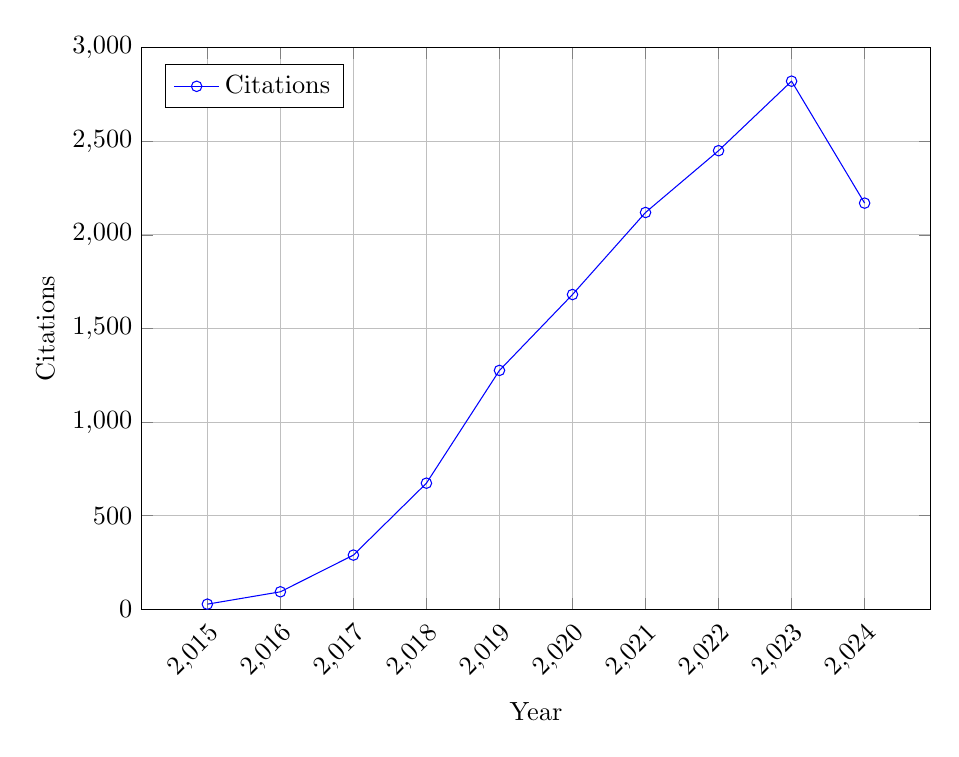
\begin{tikzpicture}[scale=0.95]
    \begin{axis}[
        width=\textwidth,
        height=0.75\textwidth,
        xlabel={Year},
        ylabel={Citations},
        xtick=data,
        xticklabel style={rotate=45,anchor=north east},
        ymin=0, ymax=3000,
        ytick={0,500,1000,1500,2000,2500,3000},
        grid=major,
        legend pos=north west
    ]
    \addplot[
        color=blue,
        mark=o
    ] coordinates {
        (2015,28) (2016,94) (2017,290) (2018,674) (2019,1276)
        (2020,1681) (2021,2119) (2022,2449) (2023,2820) (2024,2169)
    };
    \legend{Citations}
    \end{axis}
    \end{tikzpicture}
\end{minipage}%
\begin{minipage}{0.48\textwidth}
    \centering
    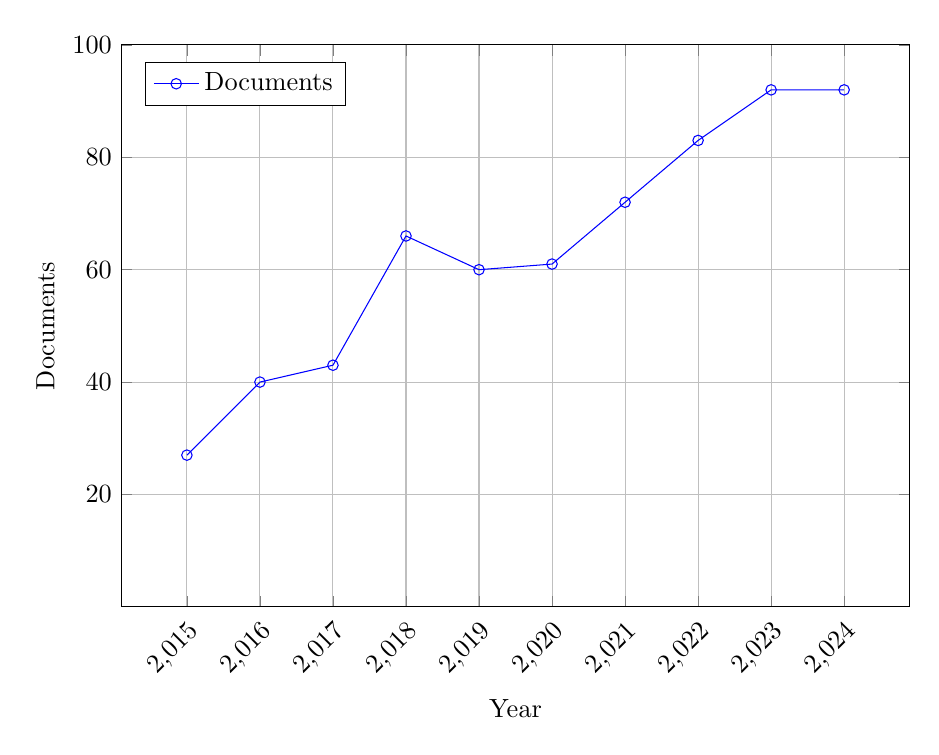
\begin{tikzpicture}[scale=0.95]
    \begin{axis}[
        width=\textwidth,
        height=0.75\textwidth,
        xlabel={Year},
        ylabel={Documents},
        xtick=data,
        xticklabel style={rotate=45,anchor=north east},
        ymin=0, ymax=100,
        ytick={20,40,60,80,100},
        grid=major,
        legend pos=north west
    ]
    \addplot[
        color=blue,
        mark=o
    ] coordinates {
    (2015,27) (2016,40) (2017,43) (2018,66) (2019,60) (2020,61) (2021,72) (2022,83) (2023,92) (2024,92)
    };
    \legend{Documents}
    \end{axis}
    \end{tikzpicture}
\end{minipage}
\caption{Review of keywords "Cryptography", "Chaos" and "Communications" search in \textit{Scopus} database.}
\end{figure}
\begin{itemize}
    \item \textbf{Mandatory:} TITLE-ABS-KEY(
    \begin{itemize}
        \item (wireless com* OR ``radio frequency'' OR rf OR ``software defined radio'' OR sdr OR transceiver OR ``digital communication'' OR ``communication systems'')
        \item AND
        \item (security OR cryptography OR encryption OR ``secure transmission'' OR ``physical layer security'')
    \end{itemize}
    \item \textbf{Classifications:} AND
    \begin{itemize}
        \item TITLE-ABS-KEY(uav\^{}2 OR drone\^{}2 OR ``unmanned aerial vehicle''\^{}2 OR vanet\^{}2 OR ``vehicular network''\^{}2 OR ``MANET'' OR ``FANET'') AND
        \item TITLE-ABS-KEY(``Chaotic Systems''\^{}3 OR ``Chaos''\^{}3 OR ``Non linear dynamics''\^{}3) AND
        \item TITLE-ABS-KEY(``FPGA''\^{}2 OR ``Programmable Logic''\^{}2 OR ``DSP''\^{}2 OR ``Circuits and Systems''\^{}3 OR ``SoC''\^{}2) AND
        \item TITLE-ABS-KEY(``spread spectrum''\^{}3 OR ofdm\^{}3 OR ``orthogonal frequency division multiplexing''\^{}3 OR mimo\^{}3 OR ``multiple-input multiple-output''\^{}3 OR ``frequency hopping''\^{}3 OR cdma\^{}3 OR ``code division multiple access''\^{}3)\^{}0.5
    \end{itemize}
\end{itemize}



\begin{table}[h!]]
\centering
\label{table}
\resizebox{\textwidth}{!}{
\begin{tabular}{|l|l|p{6cm}|p{5cm}|l|}
\hline
\textbf{Scientific Base} & \textbf{Citation} & \textbf{Article Title} & \textbf{Journal Name} & \textbf{Qualis} \\\hline
         Scopus &         3 & Optimization of Full-Duplex UAV Secure Communication \cite{} &                                             Drones  & A3 \\ \hline
         Scopus &        27 & UAV Detection and Localization Based on Multi-Directional Antennas &                               IEEE Sensors Journal & A1 \\\hline
         Scopus &        15 & Trajectory and Transmit Power Optimization for UAV Networks &          IEEE Transactions on Vehicular Technology & A1 \\\hline
         Scopus &         6 & Secure beamforming design for the UAV-enabled transmission network & Eurasip Journal on Wireless Communications and Networking  & A4 \\\hline
         Scopus &        13 & Joint obstacle avoidance and 3D deployment for UAV networks &                                        IEEE Access & A3\\\hline
         Scopus &        39 & Intelligent reflecting surface and UAV assisted secure communication &          IEEE Transactions on Vehicular Technology & A1\\\hline
         Scopus &        17 & Feature article: Security vulnerabilities of cyber-physical UAV systems &     IEEE Aerospace and Electronic Systems Magazine & A2 \\\hline
         Scopus &        39 & Energy-efficient trajectory design for secure UAV communication &                           Vehicular Communications  & A1\\\hline
\end{tabular}
}
\label{tab:1}


\end{table}



\section{Related Work}
\label{sec:Rel-Work}

Chaos-based encryption harnesses the apparent randomness inherent in mathematical chaotic models to generate keystreams. These models range from simple one-dimensional maps like the logistic map \cite{Singh.2023b}, to more complex systems such as the Lorenz \cite{Nguyen.2022}. Various techniques are utilized in conjunction with chaotic systems to enhance unpredictability and optimize the performance of chaos-based cryptography.

However, one challenge in chaos-based cryptography arises from quantization errors introduced during the simulation of chaotic systems on finite-precision computers, leading to periodic and bounded solutions. To mitigate this issue, various strategies have been proposed, including restructuring computing architectures through combinations or cascading techniques, implementing rule-defined switching mechanisms, and introducing pseudo-random variations in inputs \cite{Alawida.2024}. While these approaches have shown promise, their practical implementation as encryption schemes is restricted by their lack of consideration for the limited resources of digital devices.

In this context, emerging chaos-based methods, combined with advancements in computer arithmetic, aim to minimize the silicon footprint. Reference \cite{DaSilva.2023} utilized the Half-Unit-Bias fixed-point format to propose a novel hardware architecture for a chaos-based pseudo-random number generator. Their approach involved bicoupling the tent map with the Bernoulli map, resulting in a significant impact on logical resources and performance. References \cite{Nardo.2019} developed simple hardware designs for chaotic maps using basic logic elements such as shift registers and XOR gates, showcasing potential applications across various chaos-based systems.

Finite-precision and quantization errors play a pivotal role in the efficiency of SoC designs and are associated with the random-like behavior of systems. \cite{Tutueva.2021} demonstrated that finite-precision and discretization techniques significantly affect the robustness of chaos-based PRNGs). Additionally, \cite{Nepomuceno.2019} introduced a fresh perspective on chaos-based symmetric encryption by proposing a stream-cipher based on the lower-bound error concept, derived from two natural interval extensions of the logistic map. Subsequently, \cite{Zhou.2023} expanded upon this concept by presenting a novel framework for generating new chaotic signals utilizing the limited precision of computers.
Recently, \cite{Lima.2023} conducted a preliminary investigation into a stream-cipher based on the lower-bound error theorem, employing high-level synthesis tools in conjunction with a fourth-order Runge-Kutta method. The resultant hardware showcased the potential for parallel processing within resource-constrained devices. This paper builds upon their findings and extends the scope of their research.
\section{Preliminary Concepts}
The randomness of computing PRNG is tied to chaotic systems, perhaps more than we are aware \cite{Herring.1989}. The true nature of chaotic systems is intrinsically erratic and sensitive to initial conditions, which makes them perfectly adequate for use in encryption schemes.
These systems are obtained by natural phenomena like biochemical reactions \cite{Pu.2020} and weather forecasts \cite{Lin.2024}. It is also possible to assume much more cohesive formats, like 1-D maps such as the logistic map \cite{May.1976g0uk}. Complex dynamics of chaotic systems are observed in many environments but its behaviour is mainly studied in numerical models.

In the context of cryptography and security, chaotic systems offer unique properties that can be leveraged for encryption purposes. One such system that has garnered significant attention is the chaotic Chua's circuit. This circuit comprises four linear components: a resistor ($R$), an inductor ($L$), and two capacitors ($C_1$ and $C_2$), all interconnected by Chua's piecewise linear diode ($D$). The dynamics of this system are elucidated in \cite{Nardo.2019}.

\subsection{Finite-precision error}
In chaotic systems, finite-precision computational constraints make it impossible to achieve exact orbits. Instead, we work with approximations called pseudo-orbits.
\begin{definition}
A true orbit of a system modelled by $\dot{x}_n = f(x_n)$ is a sequence ${x_n} = [x_0, x_1, x_2, x_3, \ldots, x_n]$.
\end{definition}
\begin{definition}
The $m^{th}$ pseudo-orbit ${\hat{x}{m,n}} = [\hat{x}{m,0}, \hat{x}{m,1}, \ldots, \hat{x}{m,n}]$ approximates the true orbit ${x_n}$, where $|x_n-\hat{x}{m,n}| \leq \delta{m,n}$ and $\delta_{m,n} \in \mathbb{R_+}$ is the error.
\end{definition}
Pseudo-orbits provide an interval estimate of the true orbit's position. The challenge lies in quantifying the error between the pseudo-orbit and the true orbit.
\begin{definition}
A natural interval extension $F(X)$ of $f(x)$ satisfies $F(X) = f(x)$, where $X = [\underline{X},\overline{X}]$ is a closed interval of real numbers.
\end{definition}
Natural interval extensions can lead to different computational outcomes due to finite-precision errors. Consider these examples from Chua's circuit:
\begin{equation}
C_1 \dfrac{dV_{C_1}}{dt} = \dfrac{V_{C_2} - V_{C_1}}{R} - I_{D},
\label{eq:Extension1}
\end{equation}
\begin{equation}
C_1 \dfrac{dV_{C_1}}{dt} = \dfrac{V_{C_2}}{R} - \dfrac{V_{C_1}}{R} - I_{D}.
\label{eq:Extension2}
\end{equation}
These equations are mathematically equivalent but can produce divergent results due to finite-precision errors in digital systems.
\begin{definition}[Lower Bound Error]
The lower-bound error $\delta_{\alpha,n}$ between two pseudo-orbits ${\hat{x}{a,n}}$ and ${\hat{x}{b,n}}$ is:
\begin{equation}
\delta_{\alpha,n} = \dfrac{|\hat{x}{a,n} - \hat{x}{b,n}|}{2}.
\label{eq:LBE}
\end{equation}
\end{definition}
The lower-bound error quantifies the difference between digital arithmetical dynamical systems (pseudo-orbits) and the true orbit. This concept is crucial for understanding the behaviour of chaotic systems in digital implementations and forms the basis for the encryption scheme proposed in this dissertation.
\begin{figure}[ht!]
\centering
% This file was created by matlab2tikz.
%
%The latest updates can be retrieved from
%  http://www.mathworks.com/matlabcentral/fileexchange/22022-matlab2tikz-matlab2tikz
%where you can also make suggestions and rate matlab2tikz.
%
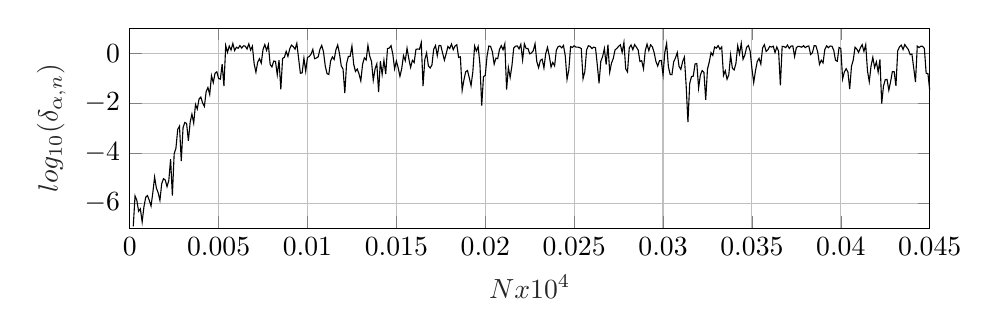
\begin{tikzpicture}

\begin{axis}[%
width=4in,  
height=1.0in,
scale only axis,
unbounded coords=jump,
clip=false,
xmin=0,
xmax=450,
xtick={0,50,100,150,200,250,300,350,400,450},
xticklabels={{0},{0.005},{0.01},{0.015},{0.02},{0.025},{0.03},{0.035},{0.04},{0.045}},
xlabel style={font=\color{white!15!black}},
xlabel={$N$$\text{x10}^\text{4}$},
ymin=-7,
ymax=1,
ylabel style={font=\color{white!15!black}},
ylabel={$log_{10}(\delta_{\alpha,n})$},
axis background/.style={fill=white},
grid=both,  % This line adds the grid  
%grid style={line width=.1pt, draw=gray!10},  % This line styles the grid  
]  
]
\addplot [color=black, forget plot]
  table[row sep=crcr]{%
1	-inf\\
2	-6.92369\\
3	-5.706206\\
4	-5.882297\\
5	-6.32163\\
6	-6.22472\\
7	-6.747599\\
8	-6.145539\\
9	-5.762322\\
10	-5.693241\\
11	-5.882297\\
12	-6.110776\\
13	-5.581267\\
14	-4.952878\\
15	-5.392211\\
16	-5.581267\\
17	-5.882297\\
18	-5.21612\\
19	-5.0206\\
20	-5.072432\\
21	-5.338229\\
22	-5.084841\\
23	-4.236384\\
24	-5.693241\\
25	-4.026888\\
26	-3.797884\\
27	-3.052643\\
28	-2.913666\\
29	-4.313562\\
30	-2.978714\\
31	-2.770515\\
32	-2.809179\\
33	-3.500608\\
34	-2.758386\\
35	-2.433345\\
36	-2.792874\\
37	-2.049505\\
38	-2.232861\\
39	-1.831134\\
40	-1.755051\\
41	-1.988404\\
42	-2.129035\\
43	-1.536343\\
44	-1.372201\\
45	-1.650367\\
46	-0.901419\\
47	-1.176616\\
48	-0.801462\\
49	-0.740918\\
50	-1.009725\\
51	-1.035858\\
52	-0.434091\\
53	-1.314646\\
54	0.307777\\
55	0.036858\\
56	0.287395\\
57	0.127877\\
58	0.387029\\
59	0.107729\\
60	0.238518\\
61	0.195502\\
62	0.306249\\
63	0.206979\\
64	0.295601\\
65	0.284448\\
66	0.167546\\
67	0.377087\\
68	0.124898\\
69	0.277603\\
70	-0.42276\\
71	-0.758798\\
72	-0.353462\\
73	-0.218711\\
74	-0.395041\\
75	0.154824\\
76	0.345121\\
77	0.112213\\
78	0.346451\\
79	-0.451436\\
80	-0.548541\\
81	-0.314136\\
82	-0.325381\\
83	-0.863414\\
84	-0.276911\\
85	-1.449128\\
86	-0.207932\\
87	-0.164652\\
88	0.075325\\
89	-0.125973\\
90	0.174432\\
91	0.324517\\
92	0.261686\\
93	0.160734\\
94	0.396788\\
95	-0.208415\\
96	-0.8007\\
97	-0.788022\\
98	-0.196734\\
99	-0.721023\\
100	-0.165982\\
101	-0.133525\\
102	-0.035948\\
103	0.151586\\
104	-0.219213\\
105	-0.192065\\
106	-0.14822\\
107	0.155607\\
108	0.313859\\
109	0.059941\\
110	-0.512666\\
111	-0.818918\\
112	-0.851384\\
113	-0.312395\\
114	-0.147638\\
115	-0.252343\\
116	0.136157\\
117	0.331383\\
118	-0.01606\\
119	-0.505548\\
120	-0.637792\\
121	-1.592337\\
122	-0.406293\\
123	-0.131757\\
124	-0.12334\\
125	0.288295\\
126	-0.444442\\
127	-0.728308\\
128	-0.632074\\
129	-0.831871\\
130	-1.105561\\
131	-0.437397\\
132	-0.185339\\
133	-0.271644\\
134	0.315084\\
135	-0.110652\\
136	-0.323887\\
137	-1.08065\\
138	-0.631936\\
139	-0.423781\\
140	-1.556686\\
141	-0.313543\\
142	-0.849916\\
143	-0.283483\\
144	-0.832166\\
145	0.18483\\
146	0.207078\\
147	0.303777\\
148	-0.040341\\
149	-0.623121\\
150	-0.312912\\
151	-0.579136\\
152	-0.923754\\
153	-0.618004\\
154	-0.097151\\
155	-0.295308\\
156	0.199702\\
157	-0.221612\\
158	-0.566436\\
159	-0.281822\\
160	-0.372353\\
161	0.151895\\
162	0.168606\\
163	0.159751\\
164	0.425214\\
165	-1.310461\\
166	-0.252165\\
167	0.013834\\
168	-0.505526\\
169	-0.591541\\
170	-0.468662\\
171	0.163853\\
172	0.308217\\
173	-0.095781\\
174	0.313413\\
175	0.302174\\
176	0.003912\\
177	-0.276791\\
178	-0.022888\\
179	0.27125\\
180	0.186027\\
181	0.36768\\
182	0.140436\\
183	0.287158\\
184	0.33959\\
185	-0.168068\\
186	-0.14365\\
187	-1.484177\\
188	-1.066038\\
189	-0.743382\\
190	-0.690334\\
191	-0.978096\\
192	-1.296547\\
193	-0.749483\\
194	0.28924\\
195	0.089096\\
196	0.269718\\
197	-0.445168\\
198	-2.095268\\
199	-0.93795\\
200	-0.886522\\
201	-0.117297\\
202	0.287788\\
203	0.275747\\
204	0.059251\\
205	-0.436559\\
206	-0.197076\\
207	-0.215721\\
208	0.149809\\
209	0.303561\\
210	0.140484\\
211	0.374547\\
212	-1.453316\\
213	-0.571448\\
214	-0.967996\\
215	-0.50064\\
216	0.206038\\
217	0.28073\\
218	0.292459\\
219	0.17578\\
220	0.356393\\
221	-0.264363\\
222	0.376893\\
223	0.183596\\
224	0.188014\\
225	-0.026003\\
226	0.009825\\
227	0.103066\\
228	0.377779\\
229	-0.340539\\
230	-0.578424\\
231	-0.285133\\
232	-0.238144\\
233	-0.589876\\
234	-0.021272\\
235	0.234324\\
236	-0.104864\\
237	-0.552677\\
238	-0.370544\\
239	-0.503371\\
240	0.13021\\
241	0.263844\\
242	0.289298\\
243	0.213807\\
244	0.309343\\
245	-0.105841\\
246	-1.045168\\
247	-0.663158\\
248	0.265851\\
249	0.233374\\
250	0.297048\\
251	0.245814\\
252	0.246192\\
253	0.229117\\
254	0.186628\\
255	-1.021147\\
256	-0.738203\\
257	0.135212\\
258	0.298785\\
259	0.273181\\
260	0.186513\\
261	0.244803\\
262	0.218682\\
263	-0.455898\\
264	-1.201469\\
265	-0.320279\\
266	-0.139123\\
267	0.188873\\
268	-0.455373\\
269	0.345658\\
270	-0.760674\\
271	-0.394558\\
272	-0.211096\\
273	0.133493\\
274	0.189765\\
275	0.275983\\
276	0.336889\\
277	0.033125\\
278	0.426544\\
279	-0.623566\\
280	-0.747898\\
281	0.216943\\
282	0.330571\\
283	0.142827\\
284	0.344081\\
285	0.245313\\
286	0.129605\\
287	-0.329537\\
288	-0.299639\\
289	-0.621658\\
290	0.101798\\
291	0.364346\\
292	0.10375\\
293	0.335475\\
294	0.257936\\
295	0.022342\\
296	-0.3319\\
297	-0.513047\\
298	-0.300071\\
299	-0.292872\\
300	-0.865111\\
301	0.033803\\
302	0.395233\\
303	-0.535108\\
304	-0.850298\\
305	-0.858129\\
306	-0.334993\\
307	-0.190919\\
308	0.02487\\
309	-0.531211\\
310	-0.647229\\
311	-0.339962\\
312	-0.157925\\
313	-1.290761\\
314	-2.751963\\
315	-1.211017\\
316	-0.935366\\
317	-0.915173\\
318	-0.429123\\
319	-0.413796\\
320	-1.392637\\
321	-0.872769\\
322	-0.69324\\
323	-0.763667\\
324	-1.864873\\
325	-0.632306\\
326	-0.34674\\
327	0.024049\\
328	-0.088254\\
329	0.248589\\
330	0.204318\\
331	0.303985\\
332	0.15617\\
333	0.252832\\
334	-0.891506\\
335	-0.701903\\
336	-1.039842\\
337	-0.859254\\
338	-0.074912\\
339	-0.601374\\
340	-0.667088\\
341	-0.404738\\
342	0.295778\\
343	-0.02905\\
344	0.393852\\
345	-0.24101\\
346	-0.076743\\
347	0.233146\\
348	0.31043\\
349	0.08133\\
350	-0.614311\\
351	-1.174582\\
352	-0.698577\\
353	-0.32855\\
354	-0.206486\\
355	-0.43441\\
356	0.213871\\
357	0.338748\\
358	0.068817\\
359	0.14094\\
360	0.273239\\
361	0.24609\\
362	0.282413\\
363	0.026714\\
364	0.248725\\
365	0.078613\\
366	-1.282672\\
367	0.275815\\
368	0.266484\\
369	0.223804\\
370	0.327278\\
371	0.191557\\
372	0.285481\\
373	0.292539\\
374	-0.13494\\
375	0.224884\\
376	0.276902\\
377	0.266187\\
378	0.24077\\
379	0.301899\\
380	0.224421\\
381	0.275391\\
382	0.289078\\
383	-0.050098\\
384	0.017527\\
385	0.303412\\
386	0.294971\\
387	0.044578\\
388	-0.444323\\
389	-0.280542\\
390	-0.388043\\
391	0.148461\\
392	0.296612\\
393	0.221356\\
394	0.287897\\
395	0.278377\\
396	0.124211\\
397	-0.278635\\
398	-0.323062\\
399	0.229622\\
400	0.190689\\
401	-1.027489\\
402	-0.747877\\
403	-0.61763\\
404	-0.754062\\
405	-1.431498\\
406	-0.521227\\
407	-0.268059\\
408	0.243165\\
409	0.163061\\
410	0.034069\\
411	0.216412\\
412	0.341776\\
413	0.073925\\
414	0.338614\\
415	-0.707099\\
416	-1.1386\\
417	-0.51403\\
418	-0.16678\\
419	-0.570645\\
420	-0.345383\\
421	-0.755541\\
422	-0.247445\\
423	-2.010926\\
424	-1.316497\\
425	-1.056455\\
426	-1.048835\\
427	-1.481561\\
428	-1.135578\\
429	-0.734501\\
430	-0.735988\\
431	-1.306737\\
432	0.096037\\
433	0.254463\\
434	0.322167\\
435	0.150057\\
436	0.34789\\
437	0.240269\\
438	0.146907\\
439	-0.058106\\
440	-0.032345\\
441	-0.590186\\
442	-1.1512\\
443	0.283086\\
444	0.226251\\
445	0.279091\\
446	0.276314\\
447	0.189986\\
448	-0.798435\\
449	-0.814957\\
450	-1.480918\\
};
\end{axis}
\end{tikzpicture}%
\caption{Lower-bound error progression in Chua's circuit for single and double precision IEEE-754 floating-point formats. Errors propagate until is no longer representable, marking a threshold for erratic behaviour usable as an encryption keystream.}
\label{fig:lower-bound-error}
\end{figure}
Figure \ref{fig:lower-bound-error} illustrates how the lower-bound error progresses during Chua's circuit execution, considering the extensions of \ref{eq:Extension1} and \ref{eq:Extension2}. This demonstrates the accumulation of uncertainties in the numerical model, which we leverage for encryption.


% ------------------------------------------------------------------------
% ELEMENTOS PÓS-TEXTUAIS
% ------------------------------------------------------------------------
\postextual
% ------------------------------------------------------------------------

% ---
% Referências bibliográficas
% ---
% Arquivo com as referências bibliográficas
\bibhang{2.2em} % Recuo da margem esquerda da lista de referências
\bibliography{unbtex-example/referencias} % O estilo de citação é selecionado automaticamente
% ---

% ---
% Apêndices
% ---
%\begin{apendicesenv}

% Imprime uma página indicando o início dos apêndices
%\partapendices

%\end{apendicesenv}
% ---

% ---
% Anexos
% ---
%\begin{anexosenv}

% Imprime uma página indicando o início dos anexos
%\partanexos

%\include{unbtex-example/anexo-a}

%\include{unbtex-example/anexo-b}

%\end{anexosenv}
% ---

\end{document}